\documentclass[
    notheorems,
    11pt,
    compress,
    aspectratio=169
]{beamer}

%\documentclass[a4paper,11pt]{article}
%\usepackage{beamerarticle}

\mode<presentation>{
    \usetheme{Madrid}
    \usecolortheme{orchid}
    \usefonttheme[onlymath]{serif}
    \setbeamertemplate{blocks}[rounded][shadow=true]
    \setbeamertemplate{navigation symbols}{}
    \setbeamertemplate{enumerate items}[square]
}

\only<article>{
    \usepackage[margin=1in]{geometry}
    \setlength{\baselineskip}{15pt}
}

\only<presentation>{
    \setlength{\baselineskip}{15pt}
}

\usepackage{config}

\graphicspath{{./figures/}}
\bibliography{bibliography.bib}

\tikzstyle{startstop} = [rectangle, rounded corners, minimum width=3cm, minimum height=1cm, text centered, draw=black, fill=red!30]

\tikzstyle{io} = [trapezium, trapezium left angle=70, text width=3cm, trapezium right angle=110, minimum width=3cm, minimum height=1cm, text centered, draw=black, fill=blue!30]

\tikzstyle{process} = [rectangle, minimum width=3cm, text width=4cm, minimum height=1cm, text centered, draw=black, fill=orange!30]

\tikzstyle{decision} = [diamond, minimum width=3cm, minimum height=1cm, text centered, draw=black, fill=green!30]

\tikzstyle{arrow} = [thick, ->, >=stealth]

% -----

\title[Codifichiamo gli algoritmi con i flow-chart]{Dal problema al programma: le basi della programmazione}
\subtitle{Codifichiamo gli algoritmi con i flow-chart}
\author{prof. Leonardo Essam Dei Rossi}
\institute[]{ITT "M. Buonarroti" - Trento (TN)}
\date[A.S. 2025/2026]{Anno scolastico 2025/2026}

% -----

\begin{document}

\begin{frame}
    \titlepage
\end{frame}

\only<presentation>{
    \begin{frame}{Indice}
        \tableofcontents
    \end{frame}
}

\only<article>{
    \maketitle
}

% -----

\section{I diagrammi a blocchi (o flow-chart)}

\begin{frame}
    \only<presentation>{
        \frametitle{I diagrammi a blocchi (o flow-chart) (1)}
    }

    \only<article>{
        \frametitle{Introduzione}
    }

    \textbf{Esistono diversi modi per scrivere un algoritmo.} il più semplice, e anche il più diffuso, è quello che utilizza i diagrammi a blocchi (o \textit{flow-chart}, letteralmente tradotto con \textit{diagrammi di flusso}): si tratta di una rappresentazione grafica, di facile interpretazione per chiunque e molto efficace perché permette di individuare “a colpo d’occhio” la struttura dell’algoritmo.

    \pause
    \vspace{\baselineskip}

    \begin{block}{}
        Vengono utilizzati simboli grafici (chiamati \textit{blocchi}) che contengono le istruzioni: i blocchi hanno quattro forme geometriche diverse per distinguere le quattro tipologie possibili di operazioni che permettono di rappresentare tutti gli algoritmi.
    \end{block}
\end{frame}

\begin{frame}<presentation>{I diagrammi a blocchi (o flow-chart) (2)}
    Le quattro tipologie di blocchi sono:

    \begin{itemize}
        \item \textbf{Blocco di inizio/fine:} è un blocco di forma ovale che viene utilizzato solo come primo e ultimo blocco del diagramma;
    \end{itemize}

    \vspace{\baselineskip}

    \begin{columns}
        \column{0.5\textwidth}
            \begin{figure}
                \centering
        
                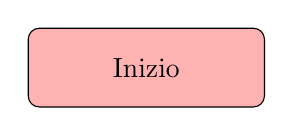
\begin{tikzpicture}[node distance=2cm]
                    \node (start) [startstop] {Inizio};
                \end{tikzpicture}
                
                \caption{Blocco di inizio}
                \label{fig:11}
            \end{figure}

        \column{0.5\textwidth}
            \begin{figure}
                \centering
        
                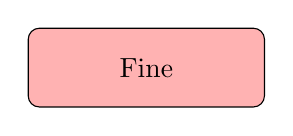
\begin{tikzpicture}[node distance=2cm]
                    \node (start) [startstop] {Fine};
                \end{tikzpicture}
                
                \caption{Blocco di fine}
                \label{fig:12}
            \end{figure}
    \end{columns}
\end{frame}

\begin{frame}<article>{Le tipologie di blocchi nei flow-chart}
    Le quattro tipologie di blocchi sono:

    \begin{itemize}
        \item \textbf{Blocco di inizio/fine:} è un blocco di forma ovale che viene utilizzato solo come primo e ultimo blocco del diagramma;
    \end{itemize}

    \begin{figure}[htbp]
        \centering
    
        \begin{minipage}{0.45\textwidth}
            \centering
            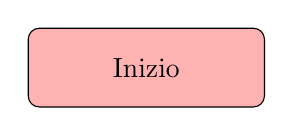
\begin{tikzpicture}[node distance=2cm]
                \node (start) [startstop] {Inizio};
            \end{tikzpicture}
            \caption{Blocco di inizio}
            \label{fig:11}
        \end{minipage}\hfill
        \begin{minipage}{0.45\textwidth}
            \centering
            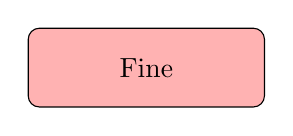
\begin{tikzpicture}[node distance=2cm]
                \node (start) [startstop] {Fine};
            \end{tikzpicture}
            \caption{Blocco di fine}
            \label{fig:12}
        \end{minipage}
    \end{figure}

    \begin{itemize}
        \item \textbf{Blocco di trasferimento di informazione (comunicazione I/O):} è un blocco a forma di parallelogramma che viene utilizzato dare/ricevere informazioni all'/dall'utente, ovvero per eseguire operazioni di \verb|INPUT| e \verb|OUTPUT|;
    \end{itemize}

    \begin{figure}[htbp]
        \centering

        \begin{tikzpicture}[node distance=2cm]
            \node (in1) [io, text width=2cm] {Input};
        \end{tikzpicture}
        
        \caption{Blocco di I/O}
        \label{fig:13}
    \end{figure}

    \begin{itemize}
        \item \textbf{Blocco di elaborazione:} è un blocco di forma rettangolare, che viene utilizzato per contenere istruzioni che effettuano trasformazione di dati;
    \end{itemize}

    \begin{figure}[htbp]
        \centering
        
        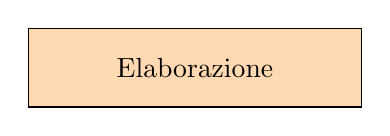
\begin{tikzpicture}[node distance=2cm]
            \node (pr1) [process] {Elaborazione};
        \end{tikzpicture}
        
        \caption{Blocco di elaborazione}
        \label{fig:14}
    \end{figure}

    \newpage

    \begin{itemize}
        \item \textbf{Blocco di decisione (condizionale):} è un blocco di forma romboidale, al suo interno vengono effettuate operazioni di confronto (te\textit{}st) che si riassumono in domande che possono avere come risultato esclusivamente due valori: SÌ oppure NO (cioè \verb|VERO| oppure \verb|FALSO|);
    \end{itemize}

    \begin{figure}[htbp]
        \centering
        
        \begin{tikzpicture}[node distance=2cm]
            \node (pr1) [decision] {Condizione};
        \end{tikzpicture}
        
        \caption{Blocco di decisione (condizionale)}
        \label{fig:15}
    \end{figure}

    Il \textbf{blocco di decisione (condizionale)} è un blocco particolare perché permette di modificare la sequenza e l'ordine di esecuzione delle istruzioni del programma.

    \begin{figure}[htbp]
        \centering

        \begin{tikzpicture}[scale=0.85, transform shape]
            \node (co1) [decision] {Condizione};

            \node (pr1) [process, below left of=co1, yshift=-1.5cm, xshift=-2cm] {Elaborazione 1};
            \node (pr2) [process, below right of=co1, yshift=-1.5cm, xshift=2cm] {Elaborazione 2};

            \draw [arrow] (co1) -| node[anchor=east] {Yes (VERO)} (pr1);
            \draw [arrow] (co1) -| node[anchor=west] {No (FALSO)} (pr2);
        \end{tikzpicture}
        
        \caption{Blocco di decisione (condizionale) ramificato}
        \label{fig:16}
    \end{figure}

    \textbf{In ogni diagramma deve essere presente un solo blocco di inizio (Figura \ref{fig:11}) e, soprattutto, un solo blocco di terminazione (Figura \ref{fig:12}):} anche se nel diagramma saranno presenti percorsi alternativi proprio in base ai risultati della istruzione di decisione, tutti i percorsi alternativi devono ricongiungersi prima della fine del diagramma.
\end{frame}

\begin{frame}<presentation>[fragile]
    \frametitle{I diagrammi a blocchi (o flow-chart) (3)}
    
    \begin{columns}
        \column{0.5\textwidth}
            \begin{itemize}
                \item \textbf{Blocco di trasferimento di informazione (comunicazione I/O):} è un blocco a forma di parallelogramma che viene utilizzato dare/ricevere informazioni all'/dall'utente, ovvero per eseguire operazioni di \verb|INPUT| e \verb|OUTPUT|;
            \end{itemize}

        \column{0.5\textwidth}
            \begin{figure}
                \centering
        
                \begin{tikzpicture}[node distance=2cm]
                    \node (in1) [io, text width=2cm] {Input};
                \end{tikzpicture}
                
                \caption{Blocco di I/O}
                \label{fig:13}
            \end{figure}
    \end{columns}
\end{frame}

\begin{frame}<presentation>[fragile]
    \frametitle{I diagrammi a blocchi (o flow-chart) (4)}
    
    \begin{columns}
        \column{0.5\textwidth}
            \begin{itemize}
                \item \textbf{Blocco di elaborazione:} è un blocco di forma rettangolare, che viene utilizzato per contenere istruzioni che effettuano trasformazione di dati;
            \end{itemize}

        \column{0.5\textwidth}
            \begin{figure}
                \centering
        
                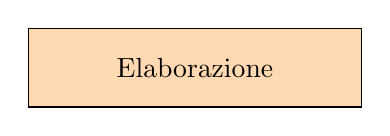
\begin{tikzpicture}[node distance=2cm]
                    \node (pr1) [process] {Elaborazione};
                \end{tikzpicture}
                
                \caption{Blocco di elaborazione}
                \label{fig:14}
            \end{figure}
    \end{columns}
\end{frame}

\begin{frame}<presentation>[fragile]
    \frametitle{I diagrammi a blocchi (o flow-chart) (5)}
    
    \begin{columns}
        \column{0.5\textwidth}
            \begin{itemize}
                \item \textbf{Blocco di decisione (condizionale):} è un blocco di forma romboidale, al suo interno vengono effettuate operazioni di confronto (te\textit{}st) che si riassumono in domande che possono avere come risultato esclusivamente due valori: SÌ oppure NO (cioè \verb|VERO| oppure \verb|FALSO|);
            \end{itemize}

        \column{0.5\textwidth}
            \begin{figure}
                \centering
        
                \begin{tikzpicture}[node distance=2cm]
                    \node (pr1) [decision] {Condizione};
                \end{tikzpicture}
                
                \caption{Blocco di decisione (condizionale)}
                \label{fig:15}
            \end{figure}
    \end{columns}
\end{frame}

\begin{frame}<presentation>{I diagrammi a blocchi (o flow-chart) (6)}
    Il \textbf{blocco di decisione (condizionale)} è un blocco particolare perché permette di modificare la sequenza e l'ordine di esecuzione delle istruzioni del programma.

    \vspace{\baselineskip}

    \begin{figure}
        \centering

        \begin{tikzpicture}[scale=0.85, transform shape]
            \node (co1) [decision] {Condizione};

            \node (pr1) [process, below left of=co1, yshift=-1.5cm, xshift=-2cm] {Elaborazione 1};
            \node (pr2) [process, below right of=co1, yshift=-1.5cm, xshift=2cm] {Elaborazione 2};

            \draw [arrow] (co1) -| node[anchor=east] {Yes (VERO)} (pr1);
            \draw [arrow] (co1) -| node[anchor=west] {No (FALSO)} (pr2);
        \end{tikzpicture}
        
        \caption{Blocco di decisione (condizionale) ramificato}
        \label{fig:16}
    \end{figure}
\end{frame}

\begin{frame}<presentation>{I diagrammi a blocchi (o flow-chart) (7)}
    \begin{block}{}
        \textbf{In ogni diagramma deve essere presente un solo blocco di inizio (Figura \ref{fig:11}) e, soprattutto, un solo blocco di terminazione (Figura \ref{fig:12}):} anche se nel diagramma saranno presenti percorsi alternativi proprio in base ai risultati della istruzione di decisione, tutti i percorsi alternativi devono ricongiungersi prima della fine del diagramma.
    \end{block}
\end{frame}

% -----

\section{Realizziamo i primi diagrammi a blocchi}

\begin{frame}
    \only<presentation>{
        \frametitle{Realizziamo i primi diagrammi a blocchi}
    }

    \only<article>{
        \frametitle{Concetti fondamentali}
    }

    Ricordiamo dalla lezione precedente \cite{2025IT100} i seguenti concetti:

    \begin{itemize}
        \item \textbf{Affrontare un problema:} per individuare la soluzione poterebbe essere necessario cercare di comprendere meglio il problema, cioè effettuare un’analisi approfondita della situazione e, nei casi più complessi, individuare una strategia risolutiva;

        \pause
        
        \item \textbf{Ricercare la strategia risolutiva:} ovvero la modalità con la quale si risolve il problema, cioè l’idea con la quale il programmatore [...] trova la “chiave di soluzione” del problema;

        \pause
        
        \item \textbf{Scomporre in istruzioni/passi:} cioè descrivere l’insieme delle operazioni (passi) che devono essere effettuati riportandoli nell’ordine in cui devono essere eseguiti (sequenza di operazioni).
    \end{itemize}
\end{frame}

% -----

\subsection{Esempio \#1: Area e perimetro di un quadrato}

\begin{frame}
    \only<presentation>{
        \frametitle{Esempio \#1: Area e perimetro di un quadrato (1)}
    }    

    Per prima cosa, definiamo la formula per calcolare il perimetro e l'area di un quadrato:

    \begin{center}
        \(P = l \cdot4\) \hspace{0.5cm} \(A = l \cdot l\)
    \end{center}

    \only<presentation>{
        \hrule
        \vspace{\baselineskip}
    }

    Realizziamo un diagramma a blocchi che descrive le operazioni necessarie per effettuare il calcolo del perimetro e dell’area di un quadrato: per prima cosa descriviamo l’algoritmo in pseudocodice e successivamente lo trasformiamo in flow-chart.

    \only<presentation>{
        \vfill
        {\usebeamercolor[fg]{structure}Tratto da:} \cite[p. 332]{ISBN_8820378434}
    }

    \only<article>{
        \vspace{\baselineskip}
    }
\end{frame}

\begin{frame}
    \only<presentation>{
        \frametitle{Esempio \#1: Area e perimetro di un quadrato (2)}
    }

    Scriviamo l'algoritmo in pseudocodifica:
    \pause
    \begin{block}{}
        \begin{enumerate}
            \item Inserisci il valore del lato;
            \pause
            \item Calcola il perimetro moltiplicando il lato per 4;
            \pause
            \item Calcola l’area moltiplicando il lato per il lato;
            \pause
            \item Visualizza il valore del perimetro e dell'area.
        \end{enumerate}
    \end{block}
\end{frame}

\begin{frame}
    \only<presentation>{
        \frametitle{Esempio \#1: Area e perimetro di un quadrato (3)}
    }

    \begin{columns}
        \column{0.4\textwidth}
        Scriviamo ora il flow-chart dell'algoritmo appena descritto:

        \column{0.6\textwidth}

        \begin{center}
            \begin{tikzpicture}[scale=0.75, transform shape]
                \node (start) [startstop] {Inizio};

                \pause
                
                \node (io1) [io, below of=start, yshift=-0.5cm] {Inserisci il lato};
                \draw [arrow] (start) -- (io1);

                \pause

                \node (pr1) [process, below of=io1, yshift=-0.5cm] {Calcola: \(P = l \cdot 4, A = l \cdot l\)};
                \draw [arrow] (io1) -- (pr1);

                % \pause

                % \node (pr2) [process, below of=pr1, yshift=-0.5cm] {Calcola: \(A = l \cdot l\)};
                % \draw [arrow] (pr1) -- (pr2);

                \pause

                \node (io2) [io, below of=pr1, yshift=-0.5cm] {Stampa: \(A\) e \(P\)};
                \draw [arrow] (pr1) -- (io2);

                \pause

                \node (end) [startstop, below of=io2, yshift=-0.5cm] {Fine};
                \draw [arrow] (io2) -- (end);
            \end{tikzpicture}
        \end{center}
    \end{columns}

    \only<article>{
        Esercizio tratto da: \cite[p. 332]{ISBN_8820378434}
    }
\end{frame}

% -----

\subsection{Esempio \#2: Quanto costa andare a scuola?}

\begin{frame}
    \only<presentation>{
        \frametitle{Esempio \#2: Quanto costa andare a scuola? (1)}
    }

    Vediamo un secondo esempio.

    \begin{block}{Quanto costa andare a scuola?}
        Calcoliamo il costo settimanale di carburante utilizzato per andare a scuola.

        \vspace{\baselineskip}
        \pause
        
        Innanzitutto individuiamo le operazioni da eseguire, cioè l’algoritmo che risolve il problema:

        \pause
        
        \begin{enumerate}
            \item Calcolare il numero di litri di benzina consumati;
            \pause
            \item Calcolare il costo totale del carburante giornaliero;
            \pause
            \item Determinare il costo settimanale.
        \end{enumerate}
    \end{block}
\end{frame}

\begin{frame}
    \only<presentation>{
        \frametitle{Esempio \#2: Quanto costa andare a scuola? (2)}
    }

    A questo punto è necessario avere a disposizione alcuni dati da fornire al programma, in modo che esso possa elaborarli.

    \vspace{\baselineskip}
    
    Questi dati, chiamati dati di ingresso (\textit{input}), sono:

    \pause
        
    \begin{enumerate}
        \item Il costo di un litro di carburante;
        \pause
        \item Il numero di chilometri tra la casa e la scuola;
        \pause
        \item Il numero di chilometri che il mezzo utilizzato effettua con un litro di carburante.
    \end{enumerate}
\end{frame}

\begin{frame}
    \only<presentation>{
        \frametitle{Esempio \#2: Quanto costa andare a scuola? (3)}

        \begin{block}{Definizione: output di un programma}
            I risultati dell’elaborazione prendono il nome di dati in uscita (o output) del programma e vengono comunicati all’utente.
        \end{block}
    
        \pause
        \vspace{\baselineskip}
    }

    \only<article>{
       \textbf{Definizione.} \textit{I risultati dell’elaborazione prendono il nome di dati in uscita (o output) del programma e vengono comunicati all’utente.}

       \vspace{\baselineskip}
    }

    In questo semplice esempio possiamo osservare come viene evidenziata la struttura generale di ogni algoritmo che possiamo schematizzare in tre fasi fondamentali: input dai dati iniziali, elaborazione mediante il programma e output dei risultati.

    \vspace{\baselineskip}

    \begin{center}
        \begin{tikzpicture}
            \node (io1) [io, text width=1cm] {Input};

            \node (el) [process, right of=io1, xshift=4cm] {Programma};
            \draw [arrow] (io1) -- (el);

            \node (io2) [io, right of=el, xshift=4cm, text width=1cm] {Output};
            \draw [arrow] (el) -- (io2);
        \end{tikzpicture}
    \end{center}
\end{frame}

\begin{frame}
    \only<presentation>{
        \frametitle{Esempio \#2: Quanto costa andare a scuola? (4)}
    }

    Una possibile codifica in pseudocodice è la seguente:

    \pause

    \begin{block}{}
        \begin{enumerate}
            \item Inserimento della distanza in km;
            \pause
            \item Inserimento del consumo in km;
            \pause
            \item Inserimento del costo del carburante al litro;
            \pause
            \item Calcolo del numero di litri consumati;
            \pause
            \item Calcolo del costo giornaliero;
            \pause
            \item Calcolo del costo settimanale;
            \pause
            \item Visualizzazione dei risultati.
        \end{enumerate}
    \end{block}
\end{frame}

\begin{frame}<presentation>[fragile]
    \frametitle{Esempio \#2: Quanto costa andare a scuola? (5)}

    \begin{columns}
        \column{0.4\textwidth}
        Parte di flow-chart per la parte di input (dall'utente):

        \column{0.6\textwidth}

        \begin{center}
            \begin{tikzpicture}[scale=0.75, transform shape]
                \node (start) [startstop] {Inizio};

                \pause

                \node (io1) [io, below of=start, yshift=-0.75cm] {Leggi: \verb|distanza_km|};
                \draw [arrow] (start) -- (io1);

                \pause

                \node (io2) [io, below of=io1, yshift=-0.75cm] {Leggi: \verb|consumo_km|};
                \draw [arrow] (io1) -- (io2);

                \pause

                \node (io3) [io, below of=io2, yshift=-0.75cm] {Leggi: \verb|costo_litro|};
                \draw [arrow] (io2) -- (io3);
            \end{tikzpicture}

            \vspace{\baselineskip}

            {\footnotesize (continua)}
        \end{center}
    \end{columns}
\end{frame}

\begin{frame}<presentation>[fragile]
    \frametitle{Esempio \#2: Quanto costa andare a scuola? (6)}

    \begin{columns}
        \column{0.4\textwidth}
        Parte di flow-chart per la parte di elaborazione:

        \column{0.6\textwidth}

        \begin{center}
            \begin{tikzpicture}[scale=0.75, transform shape]
                \node (el1) [process, below of=start, yshift=-0.75cm] {Calcola numero di litri consumati};

                \pause

                \node (el2) [process, below of=el1, yshift=-0.75cm] {Calcola il costo giornaliero};
                \draw [arrow] (el1) -- (el2);

                \pause

                \node (el3) [process, below of=el2, yshift=-0.75cm] {Calcola il costo settimanale};
                \draw [arrow] (el2) -- (el3);
            \end{tikzpicture}

            \vspace{\baselineskip}

            {\footnotesize (continua)}
        \end{center}
    \end{columns}
\end{frame}

\begin{frame}<presentation>[fragile]
    \frametitle{Esempio \#2: Quanto costa andare a scuola? (7)}

    \begin{columns}
        \column{0.4\textwidth}
        Parte di flow-chart per la parte di output (stampa a schermo):

        \column{0.6\textwidth}

        \begin{center}
            \begin{tikzpicture}[scale=0.75, transform shape]
                \node (out) [io, below of=el1, yshift=-0.75cm] {Stampa i risultati};

                % \pause

                \node (fin) [startstop, below of=out, yshift=-0.75cm] {Fine};
                \draw [arrow] (out) -- (fin);
            \end{tikzpicture}
        \end{center}
    \end{columns}
\end{frame}

\begin{frame}[fragile]
    \only<presentation>{
        \frametitle{Esempio \#2: Quanto costa andare a scuola? (8)}
    }

    \only<article>{
        Segue la rappresentazione in flow-chart:
    }

    \begin{center}
        \begin{tikzpicture}[scale=0.75, transform shape]
            \node (start) [startstop] {Inizio};
        
            \node (io1) [io, below of=start, yshift=-0.75cm] {Leggi: \verb|distanza_km|};
            \draw [arrow] (start) -- (io1);
        
            \node (io2) [io, below of=io1, yshift=-0.75cm] {Leggi: \verb|consumo_km|};
            \draw [arrow] (io1) -- (io2);
            
            \node (io3) [io, below of=io2, yshift=-0.75cm] {Leggi: \verb|costo_litro|};
            \draw [arrow] (io2) -- (io3);
        
            \node (el1) [process, right of=start, xshift=6cm] {Calcola numero di litri consumati};
        
            \draw [arrow] (io3.south) |- ++(3.5,-0.5) |- ([yshift=0.6cm]el1.north) -- (el1.north);
        
            \node (el2) [process, below of=el1, yshift=-0.75cm] {Calcola il costo giornaliero};
            \draw [arrow] (el1) -- (el2);
        
            \node (el3) [process, below of=el2, yshift=-0.75cm] {Calcola il costo settimanale};
            \draw [arrow] (el2) -- (el3);
        
        
            \node (out) [io, right of=el1, xshift=6cm] {Stampa i risultati};
        
            \draw [arrow] (el3.south) |- ++(3.2,-0.5) |- ([yshift=0.6cm]out.north) -- (out.north);
        
            \node (fin) [startstop, below of=out, yshift=-0.75cm] {Fine};
            \draw [arrow] (out) -- (fin);
        \end{tikzpicture}
    \end{center}
\end{frame}

\only<article>{
    \begin{frame}
        Su questo esempio possiamo fare alcune riflessioni:

        \begin{itemize}
            \item L’algoritmo che abbiamo scritto ha la proprietà di essere generico, ovvero che può essere utilizzato per la risoluzione di problemi simili senza che vengano specificati il tipo di automezzo utilizzato, il tipo di percorso effettuato o di carburante impiegato;
    
            \item La sequenza delle istruzioni è ordinata, cioè esiste un ordine preciso in base al quale vengono eseguite le istruzioni, che non possono essere scambiate di posto tra loro;

            \item Il numero di operazioni è finito: ciò significa che le istruzioni possono essere anche moltissime, ma non in numero infinito, altrimenti l’algoritmo non terminerebbe mai;
    
            \item Ogni operazione, inoltre, deve essere chiara, in modo che l’esecutore possa comprendere ed eseguireogni istruzione senza errori di interpretazione;
    
            \item Come precedentemente detto, è presente un solo inizio e una fine, sia che venga prodotto un risultato valido sia che non esista soluzione;

            \item I risultati generati devono essere gli stessi tutte le volte che l'algoritmo viene eseguito sugli stessi dati (determinismo), anche se dovesse essere usato un elaboratore diverso.
        \end{itemize}

        \textbf{Definizione: algoritmo deterministico.} \textit{Un algoritmo deterministico è un algoritmo dove, a parità di input, ogni passo dell’esecuzione è univocamente determinato e produce sempre la stessa sequenza di stati\footnotemark[1] fino allo stesso output finale.}

    \footnotetext[1]{Lo stato è la configurazione del programma al tempo \(t\) di esecuzione.}
    \end{frame}
}

\begin{frame}<presentation>{Esempio \#2: Quanto costa andare a scuola? (9)}
    Su questo esempio possiamo fare alcune riflessioni:

    \begin{itemize}
        \item L’algoritmo che abbiamo scritto ha la proprietà di essere generico, ovvero che può essere utilizzato per la risoluzione di problemi simili senza che vengano specificati il tipo di automezzo utilizzato, il tipo di percorso effettuato o di carburante impiegato;

        \pause

        \item La sequenza delle istruzioni è ordinata, cioè esiste un ordine preciso in base al quale vengono eseguite le istruzioni, che non possono essere scambiate di posto tra loro;
    \end{itemize}
\end{frame}

\begin{frame}<presentation>{Esempio \#2: Quanto costa andare a scuola? (10)}
    \begin{itemize}
        \item Il numero di operazioni è finito: ciò significa che le istruzioni possono essere anche moltissime, ma non in numero infinito, altrimenti l’algoritmo non terminerebbe mai;

        \pause

        \item Ogni operazione, inoltre, deve essere chiara, in modo che l’esecutore possa comprendere ed eseguireogni istruzione senza errori di interpretazione;

        \pause

        \item Come precedentemente detto, è presente un solo inizio e una fine, sia che venga prodotto un risultato valido sia che non esista soluzione;
    \end{itemize}
\end{frame}

\begin{frame}<presentation>{Esempio \#2: Quanto costa andare a scuola? (11)}
    \begin{itemize}
        \item I risultati generati devono essere gli stessi tutte le volte che l'algoritmo viene eseguito sugli stessi dati (determinismo), anche se dovesse essere usato un elaboratore diverso.
    \end{itemize}

    \pause
    \vspace{\baselineskip}

    \begin{block}{Definizione: algoritmo deterministico}
        Un algoritmo deterministico è un algoritmo dove, a parità di input, ogni passo dell’esecuzione è univocamente determinato e produce sempre la stessa sequenza di stati\footnotemark[1] fino allo stesso output finale.
    \end{block}

    \footnotetext[1]{Lo stato è la configurazione del programma al tempo \(t\) di esecuzione.}
\end{frame}

% -----

\section{Le variabili e le costanti}

\subsection{Le variabili}

\begin{frame}
    \only<presentation>{
        \frametitle{Le variabili (1)}
    }

    Nell’esempio precedente abbiamo indicato tra le operazioni il blocco che permette di effettuare la comunicazione con l’utente, cioè di descrivere le istruzioni con le quali avviene lo scambio di dati (in questo caso di numeri) che sono necessari per produrre i risultati.

    \pause
    \vspace{\baselineskip}

    In tutti i linguaggi di programmazione particolare attenzione è dedicata alle operazioni che permettono di memorizzare le informazioni in quanto i dati sono la “\textit{linfa vitale}” dell’algoritmo, poiché senza dati non può esistere l’elaborazione.
\end{frame}

\begin{frame}
    \only<presentation>{
        \frametitle{Le variabili (2)}
    }

    \only<article>{
        \vspace{\baselineskip}
    }

    Vengono messe a disposizione del programmatore le istruzioni necessarie per definire i “\textit{contenitori dei dati}” e per effettuare operazioni su di essi: questi “\textit{contenitori}”, chiamati variabili. Sono praticamente delle aree (di memoria) dove vengono “depositati” i dati prima (e dopo) le elaborazioni. Il programmatore dà a ciascuna di esse un nome (identificatore) in modo da poterle distinguere e poter in seguito fare riferimento a esse nelle istruzioni di elaborazione.

    \only<presentation>{
        \pause
        \vfill
    }

    \only<article>{
        \vspace{\baselineskip}
    }

    \begin{tabular}{@{}l l@{}}
        \textbf{Q:} & \textit{quale memoria?}
        \\
        \textbf{A:} & \textit{la memoria RAM.}
    \end{tabular}
\end{frame}

\begin{frame}
    \only<presentation>{
        \frametitle{Le variabili (3)}
    
        \begin{block}{}
            Possiamo pensare alle variabili come a dei “\textit{cassetti contenitori di dati}” posti uno vicino all’altro sui quali “\textit{attacchiamo un'etichetta}” con un nome, di fantasia oppure secondo il “\textit{buon senso}”, per ricordarci il loro contenuto e per distinguerli tra loro.
        \end{block}
    }

    \only<article>{
        \vspace{\baselineskip}
        Possiamo pensare alle variabili come a dei “\textit{cassetti contenitori di dati}” posti uno vicino all’altro sui quali “\textit{attacchiamo un'etichetta}” con un nome, di fantasia oppure secondo il “\textit{buon senso}”, per ricordarci il loro contenuto e per distinguerli tra loro.
    }
\end{frame}

\begin{frame}[fragile]
    \only<presentation>{
        \frametitle{Le variabili (4)}

        \begin{block}{Esempio}
            Se dobbiamo memorizzare il peso e l’altezza di un alunno è preferibile dare alle variabili i nomi \(\mathrm{nome}\), \(\mathrm{peso}\) e \(\mathrm{altezza}\) piuttosto che \(\mathrm{pippo}\) e \(\mathrm{paperino}\) oppure \(\mathrm{A}\) e \(\mathrm{B}\), così che direttamente dal nome della variabile (identificatore) possiamo immediatamente ricordarci cosa contiene, soprattutto se riguardiamo il programma dopo giorni o settimane!
        \end{block}
    }

    \only<article>{
        \vspace{\baselineskip}
    
        \textbf{Esempio.} Se dobbiamo memorizzare il peso e l’altezza di un alunno è preferibile dare alle variabili i nomi \textit{nome}, \textit{peso} e \textit{altezza} piuttosto che \textit{pippo} e \textit{paperino} oppure \textit{A} e \textit{B}, così che direttamente dal nome della variabile (identificatore) possiamo immediatamente ricordarci cosa contiene, soprattutto se riguardiamo il programma dopo giorni o settimane!
    }

    \vspace{\baselineskip}

    Naturalmente, tutti i nomi che attribuiamo alle variabili devono essere differenti per poterle individuare univocamente!
\end{frame}

% -----

\subsection{Esempio \#3: Secchi con l’acqua}

\begin{frame}
    \only<presentation>{
        \frametitle{Esempio \#3: Secchi con l’acqua (1)}
    }

    Si vuole descrivere l’algoritmo che permetta di versare 2 litri in un secchio della capacità di 4 litri utilizzando solo due secchi con capacità volumetrica rispettivamente di 4 e 3 litri.

    \vspace{\baselineskip}
    
    In questo esempio “abbiamo proprio bisogno” di due contenitori: sfruttiamo due variabili nelle quali inseriremo il numero dei litri presenti in ciascun secchio.

    \pause
    \vspace{\baselineskip}

    \only<presentation>{
        \begin{block}{}
            Come identificatore per queste variabili possiamo scegliere ad esempio \(\mathrm{secchio3}\) e \(\mathrm{secchio4}\), dove naturalmente con \(\mathrm{secchio3}\) indichiamo il secchio in grado di contenere 3 litri con e \(\mathrm{secchio4}\) il secondo secchio con capacità di 4 litri.
        \end{block}
    }

    \only<article>{
        Come identificatore per queste variabili possiamo scegliere ad esempio \textit{secchio3} e \textit{secchio4}, dove naturalmente con \textit{secchio3} indichiamo il secchio in grado di contenere 3 litri con e \textit{secchio4} il secondo secchio con capacità di 4 litri.
    }
\end{frame}

\only<presentation>{
    \begin{frame}{Esempio \#3: Secchi con l’acqua (2)}
        A differenza degli esempi precedenti, dove le operazioni da risolvere erano immediatamente individuate, in questo problema il procedimento è un po’ più complesso in quanto è necessario individuare una strategia risolutiva.
    
        \pause
        \vspace{\baselineskip}
    
        Osserviamo che la differenza tra i due contenitori è di 1 litro di capacità, questa quantità ci può servire per ottenere la quantità di 2 litri desiderata:
    
        \begin{enumerate}
            \item Riempio per primo il secchio da 4 litri;
            \pause
            \item Lo travaso in quello da 3 litri in modo che rimanga 1 litro nel primo secchio;
            \pause
            \item Ora svuoto il secchio da 3 litri;
            \pause
            \item Travaso il litro presente nel secchio da 4 litri in quello da 3 litri;
        \end{enumerate}
    \end{frame}
    
    \begin{frame}{Esempio \#3: Secchi con l’acqua (3)}
        \begin{enumerate}
            \setcounter{enumi}{4}
            \item Riempio nuovamente il secchio da 4 litri;
            \pause
            \item Travaso due litri in quello da 3 litri, dove 1 litro è già presente;
            \pause
            \item Nel secchio da 4 litri sono rimasti 2 litri.
        \end{enumerate}
    
        \pause
        \vspace{\baselineskip}
    
        \begin{block}{}
            Questo programma non ha né dati in input né in output ma semplicemente una sequenza di istruzioni di elaborazione in quanto i dati sono intrinsecamente indicati dal testo.
        \end{block}
    \end{frame}
}

\only<article>{
    \begin{frame}
        \vspace{\baselineskip}

        A differenza degli esempi precedenti, dove le operazioni da risolvere erano immediatamente individuate, in questo problema il procedimento è un po’ più complesso in quanto è necessario individuare una strategia risolutiva.
    
        \pause
        \vspace{\baselineskip}
    
        Osserviamo che la differenza tra i due contenitori è di 1 litro di capacità, questa quantità ci può servire per ottenere la quantità di 2 litri desiderata:
    
        \begin{enumerate}
            \item Riempio per primo il secchio da 4 litri;
            \item Lo travaso in quello da 3 litri in modo che rimanga 1 litro nel primo secchio;
            \item Ora svuoto il secchio da 3 litri;
            \item Travaso il litro presente nel secchio da 4 litri in quello da 3 litri;
            \item Riempio nuovamente il secchio da 4 litri;
            \item Travaso due litri in quello da 3 litri, dove 1 litro è già presente;
            \item Nel secchio da 4 litri sono rimasti 2 litri.
        \end{enumerate}
    
        \vspace{\baselineskip}
        
        Questo programma non ha né dati in input né in output ma semplicemente una sequenza di istruzioni di elaborazione in quanto i dati sono intrinsecamente indicati dal testo.
    \end{frame}
}

\begin{frame}
    \only<presentation>{
        \frametitle{Esempio \#3: Secchi con l’acqua (4)}
    }
    
    Ricordiamo la figura:

    \begin{center}
        \begin{tikzpicture}
            \node (io1) [io, text width=1cm] {Input};

            \node (el) [process, right of=io1, xshift=4cm] {Programma};
            \draw [arrow] (io1) -- (el);

            \node (io2) [io, right of=el, xshift=4cm, text width=1cm] {Output};
            \draw [arrow] (el) -- (io2);
        \end{tikzpicture}
    \end{center}

    \vspace{\baselineskip}

    \only<presentation>{
        \begin{center}
            \textit{Sulla base di quanto mostrato in figura, quale incongruenza si presenta rispetto all'algoritmo illustrato in precedenza?}
        \end{center}
    }

    \only<article>{
        \begin{tabular}{@{}l l@{}}
            \textbf{Q:} & \textit{quale incongruenza si presenta rispetto all'algoritmo illustrato in precedenza?}
            \\
            \textbf{A:} & \textit{la "mancanza" dell'input del programma.}
        \end{tabular}
    }
\end{frame}

\only<presentation>{
    \begin{frame}{Esempio \#3: Secchi con l’acqua (5)}
        \textbf{Non è proprio vero che non ci sono i dati di input:}\pause~in questo caso i dati di input, che sono i dati di partenza sui quali il nostro programma dovrà compiere le operazioni, sono presenti all’interno del testo del problema stesso, fanno cioè parte delle specifiche del problema.
    \end{frame}
}

\only<article>{
    \vspace{\baselineskip}
    
    In questo caso i dati di input, che sono i dati di partenza sui quali il nostro programma dovrà compiere le operazioni, sono presenti all’interno del testo del problema stesso, fanno cioè parte delle specifiche del problema.
}

\begin{frame}<presentation>{Esempio \#3: Secchi con l’acqua (6)}
    Scriviamo ora il flow-chart dell'algoritmo appena descritto:

    \vspace{\baselineskip}

    \begin{center}
        \begin{tikzpicture}[scale=0.75, transform shape]
            \node (start) [startstop] {Inizio};

            \pause

            \node (pr1) [process, below of=start, yshift=-0.5cm] {Riempi il \(\mathrm{secchio4}\)};
            \draw [arrow] (start) -- (pr1);

            \pause

            \node (pr2) [process, below of=pr1, yshift=-0.5cm] {Travasa il \(\mathrm{secchio4}\) nel \(\mathrm{secchio3}\)};
            \draw [arrow] (pr1) -- (pr2);

            \pause

            \node (pr3) [process, below of=pr2, yshift=-0.5cm] {Svuota il secchio da 3 litri};
            \draw [arrow] (pr2) -- (pr3);

            \pause
        
            \node (pr4) [process, right of=start, xshift=6cm] {Travasa il litro rimanente dal \(\mathrm{secchio4}\) al \(\mathrm{secchio3}\)};

            \pause

            \draw [arrow] (pr3.south) |- ++(3.5,-0.5) |- ([yshift=0.6cm]pr4.north) -- (pr4.north);

            \node (pr5) [process, below of=pr4, yshift=-0.75cm] {Riempi nuovamente il \(\mathrm{secchio4}\)};
            \draw [arrow] (pr4) -- (pr5);

            \pause

            \node (pr6) [process, below of=pr5, yshift=-0.75cm] {Riempi il \(\mathrm{secchio3}\) versando acqua dal \(\mathrm{secchio4}\)};
            \draw [arrow] (pr5) -- (pr6);

            \pause

            \node (io1) [io, right of=pr4, xshift=6cm, text width=4cm] {Comunica che nel \(\mathrm{secchio4}\) rimangono 2 litri d'acqua};

            \draw [arrow] (pr6.south) |- ++(3.4,-0.5) |- ([yshift=0.6cm]io1.north) -- (io1.north);

            \pause

            \node (stop) [startstop, below of=io1, yshift=-0.75cm] {Fine};
            \draw [arrow] (io1) -- (stop);
        \end{tikzpicture}
    \end{center}
\end{frame}

\only<article>{
    \newpage
}

\begin{frame}<article>
    Scriviamo ora il flow-chart dell'algoritmo appena descritto:

    \vspace{\baselineskip}

    \begin{center}
        \begin{tikzpicture}[scale=0.75, transform shape]
            \node (start) [startstop] {Inizio};

            \node (pr1) [process, below of=start, yshift=-0.5cm] {Riempi il \(\mathrm{secchio4}\)};
            \draw [arrow] (start) -- (pr1);

            \node (pr2) [process, below of=pr1, yshift=-0.5cm] {Travasa il \(\mathrm{secchio4}\) nel \(\mathrm{secchio3}\)};
            \draw [arrow] (pr1) -- (pr2);

            \node (pr3) [process, below of=pr2, yshift=-0.5cm] {Svuota il secchio da 3 litri};
            \draw [arrow] (pr2) -- (pr3);

            \node (pr4) [process, right of=start, xshift=6cm] {Travasa il litro rimanente dal \(\mathrm{secchio4}\) al \(\mathrm{secchio3}\)};

            \draw [arrow] (pr3.south) |- ++(3.5,-0.5) |- ([yshift=0.6cm]pr4.north) -- (pr4.north);

            \node (pr5) [process, below of=pr4, yshift=-0.75cm] {Riempi nuovamente il \(\mathrm{secchio4}\)};
            \draw [arrow] (pr4) -- (pr5);

            \node (pr6) [process, below of=pr5, yshift=-0.75cm] {Riempi il \(\mathrm{secchio3}\) versando acqua dal \(\mathrm{secchio4}\)};
            \draw [arrow] (pr5) -- (pr6);

            \node (io1) [io, right of=pr4, xshift=6cm, text width=4cm] {Comunica che nel \(\mathrm{secchio4}\) rimangono 2 litri d'acqua};

            \draw [arrow] (pr6.south) |- ++(3.4,-0.5) |- ([yshift=0.6cm]io1.north) -- (io1.north);

            \node (stop) [startstop, below of=io1, yshift=-0.75cm] {Fine};
            \draw [arrow] (io1) -- (stop);
        \end{tikzpicture}
    \end{center}
\end{frame}

% -----

\subsection{Le costanti}

\begin{frame}<presentation>{Le costanti (1)}
    Oltre alle necessità di memorizzare i dati che vengono elaborati nel corso dell’esecuzione del programma esistono anche delle situazioni in cui alcune variabili contengono dati che “non devono essere variati” e si mantengono uguali per tutta l’esecuzione del programma: questi dati prendono il nome di costanti e nei linguaggi di programmazione è sempre presente la possibilità di distinguerle dalle variabili, in modo che il programmatore non le modifichi, neppure per errore.
\end{frame}

\begin{frame}<presentation>{Le costanti (2)}
    \begin{block}{}
        Ad esempio tra le costanti abbiamo quelle dette “universali”, cioè che non cambiano il loro valore neppure in programmi differenti, come la velocità della luce, il valore di pi-greco (\(\pi\)), il numero dei mesi dell’anno, le ore del giorno ecc. oppure costanti temporanee che valgono solo per periodi di tempo limitato, come il valore del cambio delle monete, il costo dei beni in un supermercato, il prezzo del biglietto del cinema, il numero degli alunni di una classe ecc.
    \end{block}

    \pause
    \vspace{\baselineskip}

    Solitamente nei diagrammi di flusso non vengono indicate differenze tra variabili e costanti.
\end{frame}

\begin{frame}<article>
    Oltre alle necessità di memorizzare i dati che vengono elaborati nel corso dell’esecuzione del programma esistono anche delle situazioni in cui alcune variabili contengono dati che “non devono essere variati” e si mantengono uguali per tutta l’esecuzione del programma: questi dati prendono il nome di costanti e nei linguaggi di programmazione è sempre presente la possibilità di distinguerle dalle variabili, in modo che il programmatore non le modifichi, neppure per errore.

    \vspace{\baselineskip}

    Ad esempio tra le costanti abbiamo quelle dette “universali”, cioè che non cambiano il loro valore neppure in programmi differenti, come la velocità della luce, il valore di pi-greco (\(\pi\)), il numero dei mesi dell’anno, le ore del giorno ecc. oppure costanti temporanee che valgono solo per periodi di tempo limitato, come il valore del cambio delle monete, il costo dei beni in un supermercato, il prezzo del biglietto del cinema, il numero degli alunni di una classe ecc.

    \vspace{\baselineskip}

    Solitamente nei diagrammi di flusso non vengono indicate differenze tra variabili e costanti.
\end{frame}

% -----

\only<article>{
    \newpage
}

\section{Esercizi}

\begin{frame}
    \only<presentation>{
        \frametitle{Esercizi}
    }

    Per ciascuna delle seguenti situazioni si descriva l’algoritmo risolutivo sia in pseudocodifica che mediante flow-chart:

    \begin{enumerate}
        \item Si descriva l’algoritmo che elenca le operazioni necessarie per spedire una email allegando una fotografia;

        \item Si descriva l’algoritmo che elenca le operazioni del mattino, dalla sveglia all’uscita di casa per andare a scuola;

        \item Si descriva l’algoritmo che permette di ottenere in un contenitore 2 litri utilizzando tre contenitori rispettivamente di volume 3 litri, 6 litri e 10 litri;

        \item Si descriva l’algoritmo che permette di ottenere in un contenitore 5 litri utilizzando tre contenitori rispettivamente di volume 4 litri, 7 litri e 13 litri.
    \end{enumerate}
\end{frame}

% -----

\begin{frame}
    \only<presentation>{
        \frametitle{Riferimenti e approfondimenti}    
    }
    
    \printbibliography
\end{frame}

% -----

\end{document}
